\documentclass[18pt, a3paper, portrait]{tikzposter}
\usepackage[utf8]{inputenc}

\makeatletter
\def\title#1{\gdef\@title{\scalebox{\TP@titletextscale}{%
\begin{minipage}[t]{\linewidth}
\centering
#1
\par
\vspace{0.5em}
\end{minipage}%
}}}
\makeatother

\title{A Literature Review of Time-Series Clustering Techniques and Machine Learning Techniques Used for Monitoring of Wind Turbines}
\author{Yohann Jacob Sandvik}
\date{\today}
\institute{Institute of Electronic Systems - NTNU}
 
\usepackage{blindtext}
\usepackage{comment}
\usepackage{tikz} % To make cool diagrams
\usepackage{booktabs} % For fancy tables
\usepackage{tcolorbox} % To make colourful boxes (objectives)

\newcommand{\ra}[1]{\renewcommand{\arraystretch}{#1}} % Something about allowing more space between rows in fancy tables.
 
\usetheme{Envelope}
 
\begin{document}
 
\maketitle 

\begin{columns}
    \column{0.5}
    \block{Motivation}
    {
        To make wind power as a whole more lucrative, a good start would be to reduce the downtime,
        and improve the performance of turbines. The argument that time-series clustering may be a good approach for this is two-fold. \bigskip
        \begin{enumerate}
            \item A single wind turbine can have several sensors sampling very often, meaning that a wind
                farm can produce colossal amounts of time-series data. An unsupervised approach is
                useful because labelling of all this data is requires a lot of time and resources.
            \item When wind farms become big enough it will become too costly to manually inspect every
                turbine to construct an effective model for condition monitoring, further automation is
                required. time-series clustering is therefore a good alternative for condition monitoring.
        \end{enumerate}
    }
 
    \column{0.5}
    \block{Objectives}
    {
        \begin{tcolorbox}
            \textbf{Objectives}

            \begin{enumerate}
                \item What machine learning methods are currently being used to monitor the condition, and performance of wind turbines?
                \item What are the different methods of feature-, and model-based TSC currently used?
                \item What TSC methods are appropriate to test on time-series data produced by wind turbines? 
            \end{enumerate}
        \end{tcolorbox}
    }
\end{columns}
 
\begin{columns}
    \column{0.5}
    \block{Search terms used to find literature}
    {
        \begin{tikzfigure}
            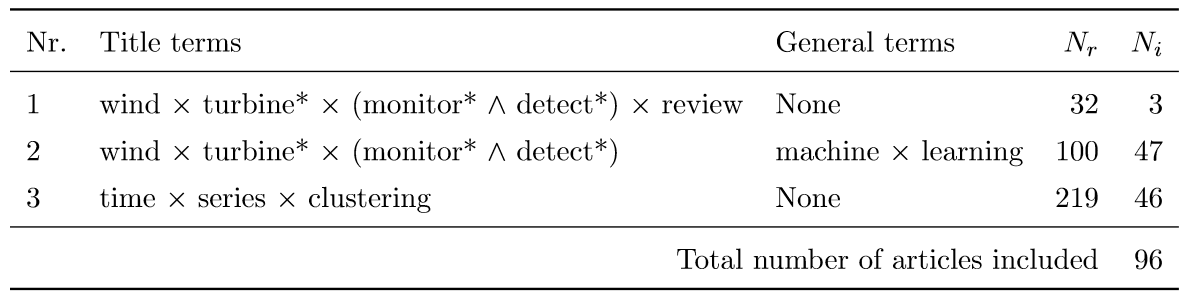
\includegraphics[width=0.45\textwidth]{images/search_terms_table.png}
        \end{tikzfigure}
    }
 
    \column{0.5}
    \block{Search term explanation}
    {
        \begin{itemize}
            \item The search engine Oria was used to search the university library of the NTNU.
            \item The \textit{Title} and \textit{General content} columns show which terms were used in the different searches; which terms where required to be in the title, and which terms could be in the ”general content”, meaning any part of the article.
            \item ''$\times$'' represents the AND operator, and ''$\wedge$'' represents the OR operator between search terms.
            \item The ''$*$'' operator means that the search will include any word beginning with the word before the star. For example detect* includes words such as detection, detecting and detected.
            \item The $N_f$ and $N_i$ columns show how many results each search yielded, and how many articles from each search were included in the review, respectively.
            \item Search 1 and 2 are used to find articles covering the first objective and search 3 is ment to cover the second objective.
        \end{itemize}
    }
\end{columns}

\block{Screening method}
{
    \begin{itemize}
        \item To make sure that the articles used were relevant, the review is limited to articles published in peer-reviewd journals, after January 2014.
        \item Search number 1 was used to find existing literature reviews on condition monitoring of wind turbines. Three good literature reviews on the subject were found so when screening the remaining articles from search 3 the focus was to find articles not included in the aforementioned reviews.
        \item When screening articles from search 3 articles meeting one (or more) of the criteria outlined in the table below were excluded from the review.
    \end{itemize}

    \begin{tikzfigure}
        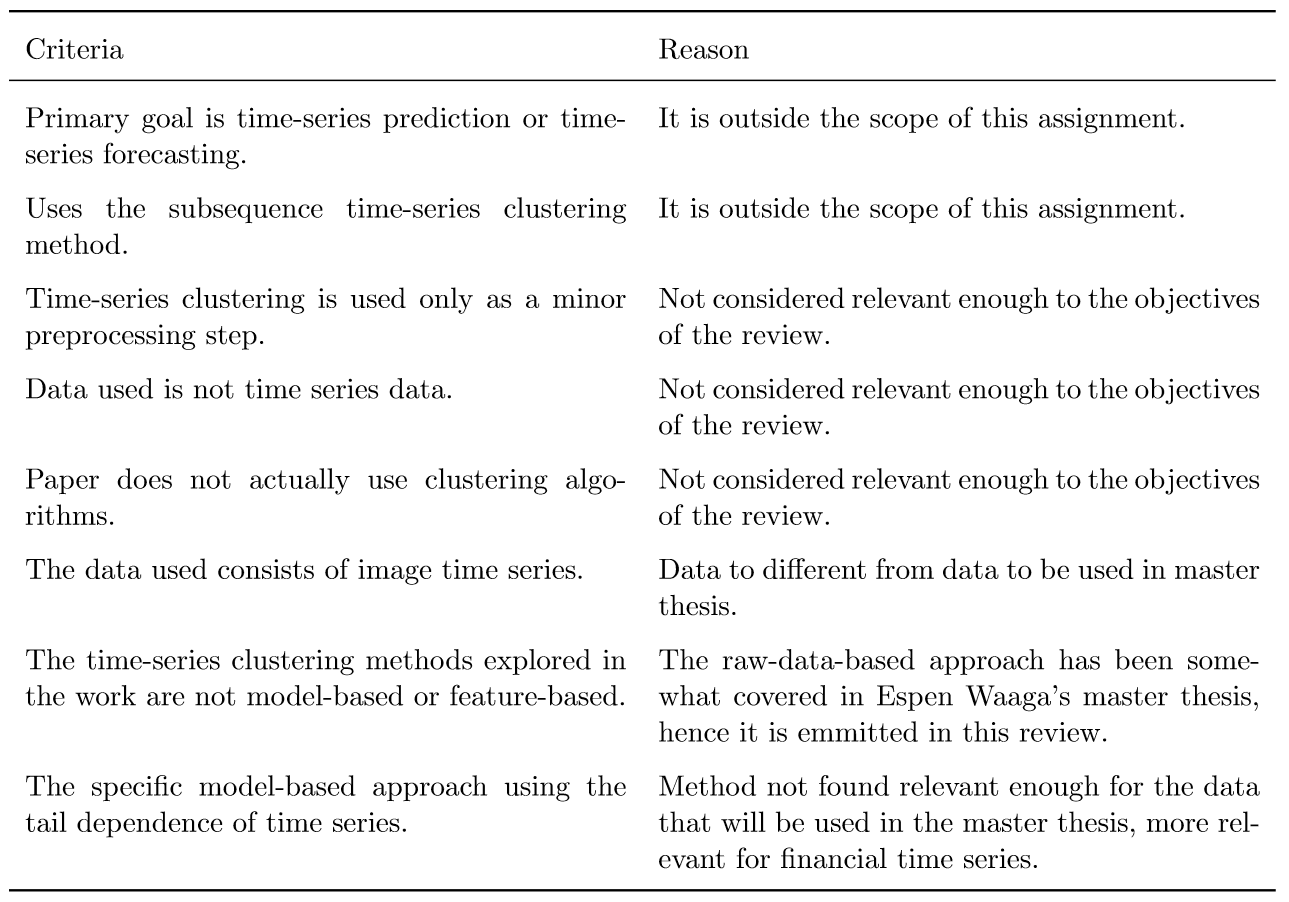
\includegraphics[width=0.5\textwidth]{images/exclusion_criteria_table.png}
    \end{tikzfigure}
}
\end{document}


